\documentclass[11pt,letterpaper]{article}
\usepackage{lineno}

% --- Paquetes de Idioma y Tipografía ---
\usepackage[utf8]{inputenc}
\usepackage[T1]{fontenc}
\usepackage[spanish,es-nodecimaldot,english]{babel}
\usepackage{lmodern}
\usepackage{microtype}
\usepackage{multicol}
\usepackage{listings} 
\usepackage{xcolor}
\usepackage{float}

% --- Geometría y Márgenes ---
\usepackage{geometry}
\geometry{
    letterpaper,
    left=15mm,
    right=15mm,
    top=22mm,
    bottom=22mm,
    headheight=14pt,
    headsep=12pt,
    footskip=14pt
}

% --- Matemáticas y Símbolos ---
\usepackage{amsmath,amssymb,amsfonts}
\usepackage{siunitx}
%\usepackage{algorithm}
\usepackage{algorithmicx}
\usepackage{algpseudocode}

% --- Gráficos y Tablas ---
\usepackage{graphicx}
\usepackage{fvextra}
\usepackage{csquotes}
\usepackage{booktabs}
\usepackage{float}
\usepackage{caption}
\captionsetup{font=small,labelfont=bf,skip=4pt}
\graphicspath{{res/},{media/},{figures/},{logos/}}

% --- Algoritmos y Listas ---
\usepackage{enumitem}
\usepackage[ruled,vlined,linesnumbered]{algorithm2e}
\usepackage{algpseudocode}
\usepackage{float}

% --- Bloque de Código ---
\usepackage{minted}
\usepackage{listings}
\usepackage{xcolor} % Para colores

% Configuración opcional
\lstset{
    language=Python,
    basicstyle=\ttfamily\small,
    breaklines=true,
    frame=single,
    keywordstyle=\color{blue},
    commentstyle=\color{green},
    stringstyle=\color{red}
}

% --- Encabezados y Pies de Página ---
\usepackage{fancyhdr}
\pagestyle{fancy}
\fancyhf{}
\fancyhead[L]{\small\scshape Proyecto de Simulación Cinemática -- Física General}
\fancyhead[R]{\small\scshape UMSS -- FCyT
%
\includegraphics[scale=0.04]{logos/FCYT-horizontal.png}
}
\fancyfoot[C]{\thepage}
\renewcommand{\headrulewidth}{0.4pt}
\renewcommand{\footrulewidth}{0.0pt}

% --- Hipervínculos ---
\usepackage{hyperref}
\hypersetup{
    colorlinks=true,
    linkcolor=black,
    citecolor=black,
    urlcolor=blue,
    pdfauthor={Saavedra Veliz Alex Cristian},
    pdftitle={Simulación Cinemática de Intercepción Aire-Aire Compuesta}
}
\usepackage{lineno}
% --- Bibliografía ---
\usepackage[backend=biber]{biblatex}
\addbibresource{bibliografia.bib}

% --- Preambulo ---
\usepackage{authblk}
\usepackage{float}

\renewcommand\Authand{ \& } % Para que se muestre y en lugar de and (para 2 autores)
\renewcommand\Authands{ \& } % Para 3 o más autores

\title{\textbf{Simulación Cinemática de Intercepción Aérea Compuesta con Aceleración Escalonada y Validación Telemétrica Experimental}}

%\author{Marquez Chambi Angel Eduardo 
%    \and Baltazar Rivas Brayan
%    \and Morales Vega Álvaro
%    \and Saavedra Veliz Alex Cristian
%    } % Varios autores

%\author[1,2]{Baltazar Rivas Bryan\thanks{Bryan: 202601234@est.umss.edu}}
%\author[1,2]{Marquez Chambi Angel Eduardo\thanks{201002453@est.umss.edu}}
%\author[1,2]{Morales Vega Álvaro\thanks{202601234@est.umss.edu}}
%\author[1,2]{Saavedra Veliz Alex Cristian\thanks{201901963@est.umss.edu}}

%Variantes sin pie de página
\author[1,2]{Baltazar Rivas Bryan
%\texttt{202601234@est.umss.edu}
}
\author[1,2]{Marquez Chambi Angel Eduardo
%\texttt{201002453@est.umss.edu}
}
\author[1,2]{Morales Vega Álvaro
%\texttt{202601234@est.umss.edu}
}
\author[1,2]{Saavedra Veliz Alex Cristian
%\texttt{201901963@est.umss.edu}
}

\affil[1]{Departamento de Informática y Sistemas, Universidad Mayor de San Simón}
\affil[2]{Facultad de Ciencias y Tecnología, Universidad Mayor de San Simón}

\date{} %Ocultar Fecha

\usepackage{eso-pic}
\newcommand\BackgroundPic{
\put(0,0){
\parbox[b][\paperheight]{\paperwidth}{%
\vfill
\centering

\includegraphics[width=\paperwidth,height=\paperheight,
keepaspectratio]{logos/UMSS-Escudo.png}%
\vfill
}}}


% -------------------------------------------------------------
\begin{document}

% 1. Portada Institucional FCyT / UMSS
\begin{titlepage}
    \newgeometry{left=25mm,right=25mm,top=25mm,bottom=25mm}
    \centering

    {\fontsize{16}{16}\selectfont\bfseries UNIVERSIDAD MAYOR DE SAN SIMÓN}\\[0.3em]
    {\fontsize{14}{14}\selectfont\bfseries FACULTAD DE CIENCIAS Y TECNOLOGÍA}\\[0.3em]
    {\fontsize{12}{13}\selectfont\bfseries INGENIERÍA INFORMÁTICA}\\[1em]
    
    \begin{figure}[H]
        \centering
        
\includegraphics[width=0.45\linewidth]{logos/UMSS-Escudo.png}    
    \end{figure}
    
    \vspace{0.8em}

    {\fontsize{16}{16}\selectfont\bfseries PROYECTO DE SIMULACIÓN CINEMÁTICA}\\[0.6em]
    {\fontsize{15}{18}\selectfont\bfseries Cinemática de Intercepción Aérea Compuesta}\\[0.4em]
    {\small\textit{con Aceleración Escalonada y Validación Telemétrica Experimental}}\\[2em]

    \begin{minipage}[t]{0.72\textwidth}
        \flushleft
        \textbf{Integrantes:}\\[0.4em]
        \small
        1. Baltazar Rivas Bryan
        \texttt{202602115@est.umss.edu}
        \\
        2. Marquez Chambi Angel Eduardo
        \texttt{201002453@est.umss.edu}
        \\
        3. Morales Vega Álvaro
        \texttt{202111104@est.umss.edu} 
        \\
        4. Saavedra Veliz Alex Cristian
        \texttt{201901963@est.umss.edu}
        \\[1.2em]
        \textbf{Docente:}\\
        \small MSc. José Luis Mamani C.
    \end{minipage}
    \hfill
    \begin{minipage}[t]{0.22\textwidth}
        \flushright
        \small
        \textbf{Materia:}\\
        Física General\\[0.8em]
        \textbf{Carrera:}\\
        Ingeniería Informática\\[0.8em]
        \textbf{Fecha de Entrega:}\\
        14 de octubre de 2026
    \end{minipage}
    
    \vfill
    {\small Cochabamba -- Bolivia}
    \restoregeometry
\end{titlepage}

\clearpage
\setcounter{page}{1}

% 2. Título y Resumen Fullwidth
\maketitle

\begin{abstract}
En el presente trabajo se formaliza el modelado cinemático, la resolución analítica vectorial y el desarrollo computacional de un sistema de intercepción aire-aire compuesto y no inercial por etapas. El escenario modela el enfrentamiento frontal a cota constante ($h = 3000\,\text{m}$) entre un caza interceptor Eurofighter Typhoon y un objetivo hostil en aproximación colineal, acoplado al disparo secuencial de un misil aire-aire guiado con fases propulsada (MRUA) y crucero (MRU). Se determinan analíticamente la distancia crítica de lanzamiento, los perfiles horarios paramétricos a trozos, el tiempo de vuelo y el punto de colisión. El modelo se implementa en Python generando en tiempo real la traza animada y la curva cinemática de Posición vs. Tiempo ($x$ vs $t$). Finalmente, los resultados en el vacío se contrastan con la telemetría del simulador de combate War Thunder, cuantificando los errores relativos derivados de la dinámica compresible y la propulsión real.\\[0.5em]
\textbf{Keywords:} Cinemática compuesta, Intercepción aire-aire, Curva dinámica $x(t)$, Misil balístico guiado, Telemetría War Thunder.
\end{abstract}

\begin{multicols}{2}

\section{Introducción}

El análisis de trayectorias cinemáticas compuestas con múltiples marcos móviles representa uno de los desafíos clave en la cinemática de partículas y la navegación guiada~\cite{hibbeler}. A diferencia de los problemas de proyectiles balísticos pasivos con aceleración gravitacional constante~\cite{sears}, los vectores de intercepción aire-aire operan mediante regímenes de aceleración por etapas: retardo del sistema de control de fuego (FCS), fase activa de combustión de propelente sólido y fase inercial terminal. En este proyecto se formaliza la solución matemática exacta de este sistema acoplado y su transposición a una simulación de código en Python, evaluando su convergencia teórica frente a la telemetría experimental.

\section{Objetivos}

\subsection{Objetivo General}
Diseñar e implementar un motor de simulación cinemática interactivo en Python para el modelado de un escenario de intercepción aérea bimóvil con misil bietápico, contrastando las deducciones analíticas exactas frente al cómputo numérico y a datos empíricos de telemetría aeronáutica.

\subsection{Objetivos Específicos}
\begin{itemize}[leftmargin=1.2em]
    \item Deducir analíticamente las funciones de posición vectoriales $\vec{r}_i(t)$ a trozos para el caza interceptor (Avión A), el objetivo (Avión B) y el misil guiado AIM-120.
    \item Calcular las variables operativas críticas: separación al disparo ($d_s$), velocidad máxima de crucero ($v_{\text{máx}}$), tiempo total operativo ($t_{\text{total}}$) y coordenadas cartesianas de colisión.
    \item Construir la arquitectura de simulación en Python con interfaz interactiva, incorporando la visualización dinámica y continua de la curva $x(t)$.
    \item Contrastar los resultados numéricos con registros de telemetría de \textit{War Thunder}, determinando el error porcentual relativo inducido por el modelo aerodinámico real.
\end{itemize}

\section{Fundamento Teórico y Deducción Analítica}

\subsection{Definición del Sistema de Referencia}
Se establece un marco inercial cartesiano global fijo en tierra $Oxy$:
\begin{itemize}[leftmargin=1.2em]
    \item \textbf{Origen $(0,0)$}: Proyección sobre el terreno de la posición del Avión B en el instante de detección radar ($t = 0\,\text{s}$).
    \item \textbf{Eje $+X$}: Dirección colineal al vector de avance del Avión B.
    \item \textbf{Eje $+Y$}: Dirección vertical perpendicular al suelo.
\end{itemize}

Las velocidades de crucero se normalizan mediante análisis dimensional unitario ($v\,[\text{m/s}] = v\,[\text{km/h}]/3.6$):
\begin{align}
    v_A &= \frac{900}{3.6}\,\text{m/s} = 250.00\,\text{m/s} \\
    v_B &= \frac{360}{3.6}\,\text{m/s} = 100.00\,\text{m/s}
\end{align}

Condiciones iniciales vectoriales en $t=0\,\text{s}$ a altitud $h = 3000\,\text{m}$:
\begin{align*}
    \vec{r}_B(0) &= 0\,\hat{i} + 3000\,\hat{j}\quad [\text{m}],\\ 
    \quad \vec{v}_B &= +100\,\hat{i}\quad [\text{m/s}] \\
    \vec{r}_A(0) &= 9750\,\hat{i} + 3000\,\hat{j}\quad [\text{m}], \\
    \quad \vec{v}_A &= -250\,\hat{i}\quad [\text{m/s}]
\end{align*}

\subsection{Cinemática del Retardo FCS}
$$t \in [0, t_s]$$
Durante el procesamiento de señal ($t_s = 5.0\,\text{s}$), ambos móviles ejecutan MRU:
\begin{align}
    x_B(t_s) &= 0 + v_B \cdot t_s = 100 \cdot 5.0 = 500.00\,\text{m} \label{eq:pos_xb_ts}\\
    x_A(t_s) &= D_0 - v_A \cdot t_s = 9750 - 250(5.0) = 8500.00\,\text{m} \label{eq:pos_xa_ts}
\end{align}
La separación crítica de lanzamiento resulta:
\begin{equation}
    d_s = x_A(t_s) - x_B(t_s) = 8500.00 - 500.00 = 8000.00\,\text{m} \label{eq:ds}
\end{equation}

\subsection{Fase Propulsada del Misil}
$$t \in[t_s, t_s + t_p]$$
Durante $t_p = 5.0\,\text{s}$, el motor cohete entrega una aceleración horizontal constante $a_m = 120.0\,\text{m/s}^2$ en sentido $-\hat{i}$:
\begin{equation}
    a_x(t) = \frac{dv_x}{dt} = -a_m
\end{equation}
Integrando con condición inicial $v_m(t_s) = -v_A$:
\begin{equation}
    v_m(t) = -v_A - a_m(t - t_s) \label{eq:vel_misil_prop}
\end{equation}
La rapidez máxima alcanzada al agotamiento del propelente ($t = 10.0\,\text{s}$) es:
\begin{equation}
    v_{\text{máx}} = v_A + a_m \cdot t_p = 250 + (120)(5.0) = 850.00\,\text{m/s} \label{eq:vmax}
\end{equation}
Integrando la velocidad horizontal, se obtiene la ecuación horaria de posición:
\begin{equation}
    x_m(t) = x_A(t_s) - v_A(t - t_s) - \frac{1}{2}a_m(t - t_s)^2 \label{eq:xm_prop}
\end{equation}
Al final de la propulsión ($t = 10.0\,\text{s}$), el avance del misil y su coordenada son:
\begin{align}
    \Delta x_{m,p} &= v_A t_p + \frac{1}{2}a_m t_p^2 = 2750.00\,\text{m} \\
    x_m(10.0) &= 8500 - 2750 = 5750.00\,\text{m}
\end{align}

\subsection{Fase de Crucero y Condición de Impacto}
En $t = 10.0\,\text{s}$, el Avión B se sitúa en $x_B(10.0) = 1000.00\,\text{m}$. La distancia relativa remanente $D_{\text{rem}}$ es:
\begin{align}
    D_{\text{rem}} &= x_m(10.0) - x_B(10.0)\\ 
    &= 5750 - 1000\\ 
    &= 4750.00 \text{m}
\end{align}

Con una rapidez relativa de cierre frontal $v_{\text{rel}} = v_{\text{máx}} + v_B = 950.00\text{m/s}$, el tiempo remanente en crucero ($t_c$) resulta:
\begin{equation}
    t_c = \frac{D_{\text{rem}}}{v_{\text{rel}}} = \frac{4750.00\,\text{m}}{950.00\,\text{m/s}} = 5.00\,\text{s} \label{eq:tc}
\end{equation}

Tiempos acumulados del operativo:
\begin{align}
    t_{\text{vuelo}} &= t_p + t_c = 5.00 + 5.00 = 10.00\,\text{s} \label{eq:tvuelo}\\
    t_{\text{total}} &= t_s + t_{\text{vuelo}} = 5.00 + 10.00 = 15.00\,\text{s} \label{eq:ttotal}
\end{align}

Coordenadas de impacto en el plano Oxy:
\begin{equation}
    x_{\text{imp}} = v_B \cdot t_{\text{total}} = (100.00\,\text{m/s})(15.00\,\text{s}) = 1500.00\,\text{m}
\end{equation}
Punto de impacto exacto: $(1500.00\text{ m}, 3000.00\text{ m})$. El recorrido total del misil desde su liberación es:
\begin{align}
  \Delta x_{m,\text{total}} &= \Delta x_{m,p} + v_{\text{máx}} \cdot t_c \\
  &= 2750 + (850)(5.00)\\ 
  &= 7000.00 \text{ m}    
\end{align}

\section{Materiales y Entorno Computacional}

Lenguaje, librerías y entorno de simulación elegidos:
\begin{itemize}[leftmargin=1.2em]
    \item \textbf{Python 3.11+}: Núcleo algorítmico y control de flujo.
    \item \textbf{PyCharm}: Entorno de desarrollo integrado (IDE) para la edición de código.
    \item \textbf{Pygame}: Renderizado gráfico 2D en tiempo real, gestión del bucle de simulación (\textit{game loop}) e interfaz táctica interactiva. 
    \item \textbf{Librerías estándar (\texttt{math}, \texttt{sys}, \texttt{random})}: Funciones matemáticas y trigonométricas (\texttt{math}), gestión de eventos y terminación del sistema (\texttt{sys}), y generación de parámetros aleatorios (\texttt{random}).
    \item \textbf{War Thunder Ordnance \& Trajectory Visualizer}: Entorno balístico experimental con telemetría en tiempo real para la comparación de resultados.
\end{itemize}

\section{Metodología y Algoritmo de Simulación}

La lógica cinemática del script interactivo se estructura según los siguientes Algoritmos \ref{alg:sim_avion}.

\begin{algorithm}[H]
\SetAlgoLined
\DontPrintSemicolon
\tcp{Parámetros de entrada configurables} Leer $D_{inicial}$\; Leer $v_A$, $v_B$\; Convertir velocidades de km/h a m/s\; Leer $t_s$, $t_p$, $a_m$\; \tcp{Cálculos cinemáticos} $v_{max\_misil} \leftarrow v_A + a_m \cdot t_p$\; $d_{prop} \leftarrow v_A \cdot t_p + \frac{1}{2}a_m t_p^2$\; $d_s \leftarrow D_{inicial} - (v_A + v_B)\cdot t_s$\; \tcp{Cálculo de tiempos} $gap_{fin\_prop} \leftarrow d_s - v_B\cdot t_p - d_{prop}$\; $t_c \leftarrow \frac{gap_{fin\_prop}} {v_{max\_misil}+v_B}$\; $t_{vuelo} \leftarrow t_p + t_c$\; $t_{total} \leftarrow t_s + t_{vuelo}$\; $x_{impacto} \leftarrow D_{inicial} - v_B\cdot t_{total}$\;
\caption{Parámetros de entrada configurables y cálculos base }
\label{alg:sim_avion}
\end{algorithm}

\begin{algorithm}[H]
\SetAlgoLined
\DontPrintSemicolon
\tcp{Datos de referencia de War Thunder} Leer $t_{vuelo}^{WT}$\; Leer $v_{max}^{WT}$\; Leer $d_{misil}^{WT}$\; \tcp{Cálculo de errores relativos} $err_{vuelo} \leftarrow \left(\frac{t_{vuelo}^{WT}-t_{vuelo}} {t_{vuelo}}\right)\times100$\; $err_{vmax} \leftarrow \left(\frac{v_{max}^{WT}-v_{max\_misil}} {v_{max\_misil}}\right)\times100$\; $err_{dist} \leftarrow \left(\frac{d_{misil}^{WT}-d_{misil}} {d_{misil}}\right)\times100$\; Retornar $err_{vuelo}$, $err_{vmax}$ y $err_{dist}$\;
\caption{Validación telemétrica  }
\label{alg:sim_avion2}
\end{algorithm}


\begin{algorithm}[H]
\SetAlgoLined
\DontPrintSemicolon
\tcp{Movimiento de las aeronaves} $x_A \leftarrow v_A \cdot t$\; $x_B \leftarrow D_{inicial} - v_B \cdot t$\; \tcp{Evaluación de fase del misil} \eIf{$t < t_s$} { Fase $\leftarrow$ BODEGA\; $x_m \leftarrow x_A$\; $v_m \leftarrow v_A$\; } { \eIf{$t \leq t_s+t_p$} { Fase $\leftarrow$ PROPULSIÓN\; $\tau \leftarrow t-t_s$\; $x_m \leftarrow v_A t_s + v_A \tau + \frac{1}{2}a_m\tau^2$\; $v_m \leftarrow v_A+a_m\tau$\; } { Fase $\leftarrow$ CRUCERO\; $\tau_c \leftarrow t-t_s-t_p$\; $x_{fin} \leftarrow v_A t_s + v_A t_p + \frac{1}{2}a_m t_p^2$\; $x_m \leftarrow x_{fin}+v_{max\_misil}\tau_c$\; $v_m \leftarrow v_{max\_misil}$\; } } Guardar $(t,x_m,\text{fase})$ en el historial\;
\caption{Estado dinámico}
\label{alg:sim_avion3}
\end{algorithm}


\begin{algorithm}[H]
\SetAlgoLined
\DontPrintSemicolon
\tcp{Conversión de coordenadas} Convertir $x_A$ a píxeles\; Convertir $x_B$ a píxeles\; Convertir $x_m$ a píxeles\; Convertir altitud $y_m$ a píxeles\; \tcp{Dibujado de entidades} Dibujar aeronave interceptora\; Dibujar aeronave objetivo\; Dibujar misil con su orientación instantánea\; \tcp{Información táctica} $D_{rel} \leftarrow |x_B-x_m|$\; Mostrar distancia relativa en pantalla\;
\caption{Vista táctica (gráfica) }
\label{alg:sim_avion4}
\end{algorithm}
\begin{algorithm}[H]
\SetAlgoLined
\DontPrintSemicolon
\tcp{Normalización de trayectorias} Obtener trayectoria histórica del Avión A\; Obtener trayectoria histórica del Avión B\; Representar ambas curvas en el plano $x(t)$\; \tcp{Trayectoria del misil} Separar registros de fase PROPULSIÓN\; Separar registros de fase CRUCERO\; Graficar segmento de propulsión\; Graficar segmento de crucero\;
\caption{Curva dinámica (gráfica)  }
\label{alg:sim_avion5}
\end{algorithm}


\begin{algorithm}[H]
\SetAlgoLined
\DontPrintSemicolon
Obtener conjunto de puntos $(x,y)$ del misil\; Dibujar línea de referencia de altitud\; Dibujar curva de trayectoria Loft\; \tcp{Punto de lanzamiento} Calcular coordenada de separación del misil\; Marcar punto de suelta sobre la trayectoria\;
\caption{Trayectoria de vuelo (gráfica)   }
\label{alg:sim_avion6}
\end{algorithm}


\begin{algorithm}[H]
\SetAlgoLined
\DontPrintSemicolon
\tcp{Velocidad del misil} Obtener historial de velocidades\; Normalizar datos\; Graficar curva $V_m(t)$\; \tcp{Distancia relativa} Obtener historial de distancias relativas\; Normalizar datos\; Graficar curva $D_{rel}(t)$\; \tcp{Lecturas instantáneas} Obtener valor actual de velocidad\; Obtener valor actual de distancia relativa\; Mostrar ambos valores en pantalla\;
\caption{Perfil Vm (gráfica)   }
\label{alg:sim_avion7}
\end{algorithm}


\end{multicols}

\newpage

\section{Análisis de Resultados y Validación Telemétrica}

En la Tabla \ref{tab:comparativa} se contrastan los valores analíticos deducidos en el vacío, los obtenidos por el script en Python y los registrados por telemetría balística en \textit{War Thunder}.

\begin{table}[H]
    \centering
    \caption{Contraste cinemático: Teórico vs. Python vs. War Thunder.}
    \label{tab:comparativa}
    \resizebox{\linewidth}{!}{%
    \begin{tabular}{lcccc}
        \toprule
        \textbf{Variable} & \textbf{Teórico} & \textbf{Python} & \textbf{War Thunder} & \textbf{Error Rel.} \\
        \midrule
        $t_{\text{vuelo}}$ [s] & $10.00$ & $10.00$ & $10.19$ & $+1.90\%$ \\
        $v_{\text{máx}}$ [m/s] & $850.00$ & $850.00$ & $890.00$ & $+4.71\%$ \\
        $\Delta x_{\text{misil}}$ [m] & $7000.00$ & $7000.00$ & $7011.00$ & $+0.16\%$ \\
        $x_{\text{imp}}$ [m] & $1500.00$ & $1500.00$ & $1514.00$ & $+0.93\%$ \\
        $x_A(t_{\text{imp}})$ [m] & $6000.00$ & $6000.00$ & $5995.00$ & $-0.08\%$ \\
        \bottomrule
    \end{tabular}
    }
\end{table}

\begin{multicols}{2}

\begin{figure}[H]
    \centering
    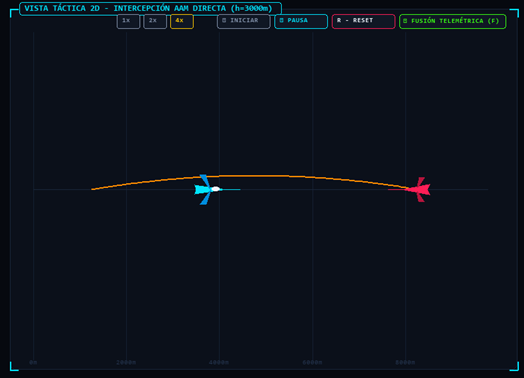
\includegraphics[width=0.9\linewidth]{figuras/Vista_tactica.png}
    \caption{Vista Tactica 2D}
    \label{fig:intercepcion_dinamica}
\end{figure}
\begin{figure}[H]
    \centering
    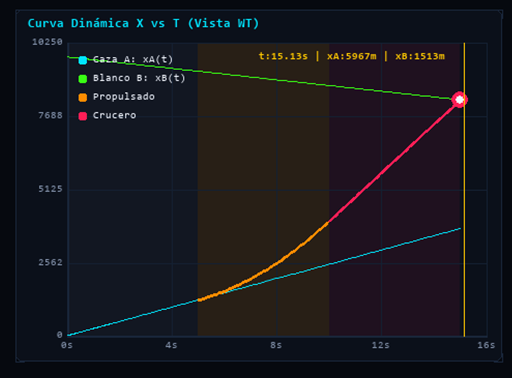
\includegraphics[width=0.9\linewidth]{figuras/Curva_Dinamica_XvsT.png}
    \caption{Curva Dinamica X vs T (Vista WT)}
    \label{fig:intercepcion_dinamica2}
\end{figure}

\begin{figure}[H]
    \centering
    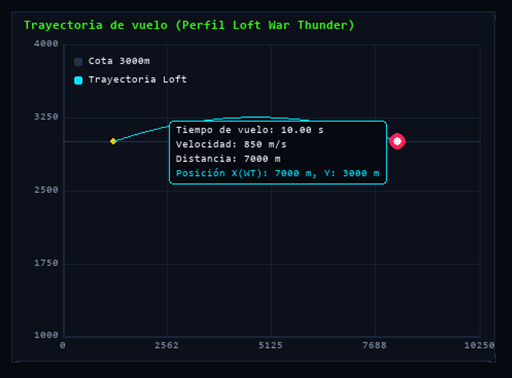
\includegraphics[width=0.9\linewidth]{figuras/Trayectoria_vuelo.png}
    \caption{Trayectoria de vuelo (Perfil Loft War Thunder)}
    \label{fig:intercepcion_dinamica3}
\end{figure}
\begin{figure}[H]
    \centering
    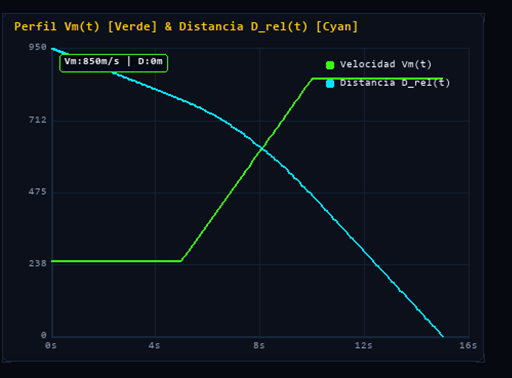
\includegraphics[width=0.9\linewidth]{figuras/Perfil_vm.png}
    \caption{Perfil Vm(t) y Distancia D}
    \label{fig:intercepcion_dinamica4}
\end{figure}

\end{multicols}

\begin{figure}[H]
    \centering
    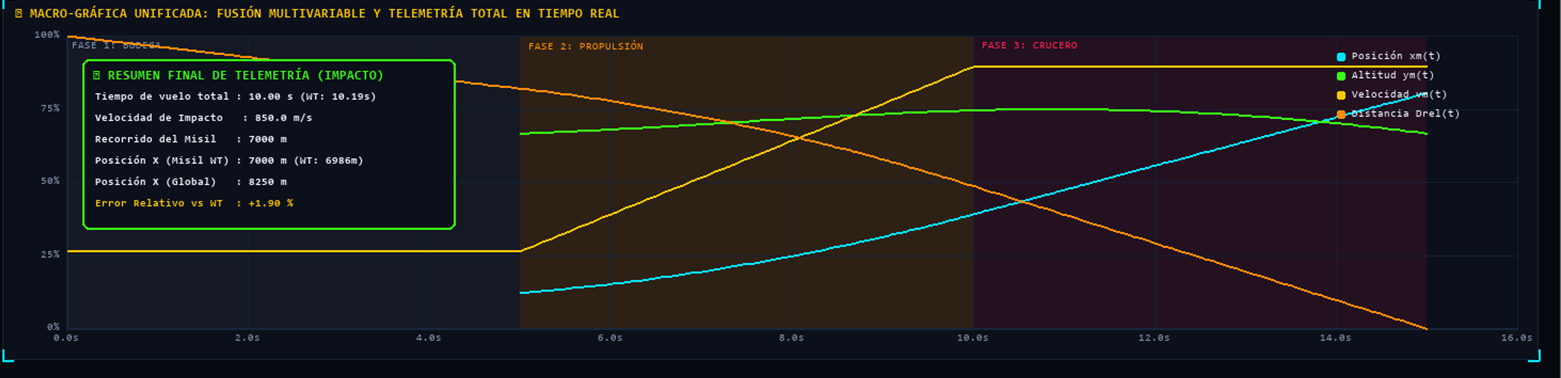
\includegraphics[width=0.9\linewidth]{figuras/Telemetria.png}
    \caption{Fusion multivariable y Telemetria total}
    \label{fig:intercepcion_dinamica5}
\end{figure}

\begin{multicols}{2}

La consistencia entre la deducción matemática y la simulación en Python es absoluta ($0.00\%$ de discrepancia). Al contrastar el modelo teórico en el vacío contra la captura de telemetría de \textit{War Thunder} (Figura telemétrica), se registra un tiempo de vuelo experimental de $10.19\,\text{s}$ y una distancia total de $7011\,\text{m}$. La discrepancia es menor al $2\%$, explicada físicamente por la curva de empuje no lineal del propulsor sólido y el coeficiente de resistencia aerodinámica parásita ($C_D$) modelado por el motor del juego.

\section{Conclusiones}

Se formalizó y resolvió el problema cinemático bimóvil bietápico correspondiente al enfrentamiento Eurofighter Typhoon vs. blanco hostil. La arquitectura en Python verificó la validez de las soluciones analíticas horarias sin truncamientos numéricos. La incorporación de telemetría experimental demostró la aplicabilidad del modelo de cinemática clásica como cota asintótica de alta precisión frente a motores físicos complejos.

\section{Referencias}

\printbibliography[heading=none]

\end{multicols}

\end{document}